\section{Experimentación y resultados}

\subsection{Resultados globales}

\begin{table}[htbp]
\centering
\caption{Resultados globales por modelo (JSON válido, exactitud estricta y laxa, latencia) y distribución de errores de la taxonomía, en las mismas doce filas. I: incorrectas; CI: confusión de intención; CD: confusión de dispositivo; CU: confusión de ubicación; VN: valor numérico incorrecto; SE: sin error semántico (equivalente por otro motivo); US: uso de sinónimos (difiere solo por un sinónimo).}
\label{tab:resultados}
{\setlength{\tabcolsep}{2pt}
{\footnotesize
\begin{tabular}{lrrrrrrrrrrr}
\toprule
Modelo & JSON & Estr. & Laxa & Lat. & I & CI & CD & CU & VN & SE & US \\
\midrule
LFM2.5-230M & 87.5 & 6.2 & 34.4 & 6.31 & 30 & 0 & 20 & 4 & 0 & 1 & 8 \\
granite-4.0-h-350m & 100.0 & 40.6 & 71.9 & 56.45 & 19 & 0 & 9 & 0 & 0 & 3 & 7 \\
LFM2.5-350M & 100.0 & 0.0 & 37.5 & 9.62 & 32 & 0 & 20 & 5 & 0 & 1 & 11 \\
granite-4.0-350m & 100.0 & 28.1 & 62.5 & 13.77 & 23 & 3 & 9 & 0 & 0 & 5 & 6 \\
SmolLM2-360M-Instruct & 25.0 & 9.4 & 93.8 & 20.47 & 29 & 0 & 2 & 0 & 0 & 1 & 26 \\
Qwen3.5-0.8B & 100.0 & 75.0 & 84.4 & 18.17 & 8 & 1 & 4 & 0 & 0 & 0 & 3 \\
OLMo-2-0425-1B-Instruct & 100.0 & 3.1 & 37.5 & 35.31 & 31 & 0 & 19 & 3 & 1 & 2 & 9 \\
LFM2.5-1.2B-Instruct & 100.0 & 56.2 & 84.4 & 31.88 & 14 & 2 & 3 & 0 & 0 & 2 & 7 \\
granite-4.0-h-1b & 100.0 & 71.9 & 96.9 & 123.14 & 9 & 0 & 1 & 0 & 0 & 7 & 1 \\
Qwen2.5-1.5B-Instruct & 100.0 & 65.6 & 93.8 & 38.13 & 11 & 0 & 1 & 1 & 0 & 2 & 7 \\
granite-4.0-1b & 100.0 & 90.6 & 100.0 & 42.78 & 3 & 0 & 0 & 0 & 0 & 1 & 2 \\
SmolLM2-1.7B-Instruct & 100.0 & 50.0 & 84.4 & 56.71 & 16 & 0 & 5 & 0 & 0 & 5 & 6 \\
\bottomrule
\end{tabular}
}
}
\end{table}


\begin{figure}[htbp]
\centering
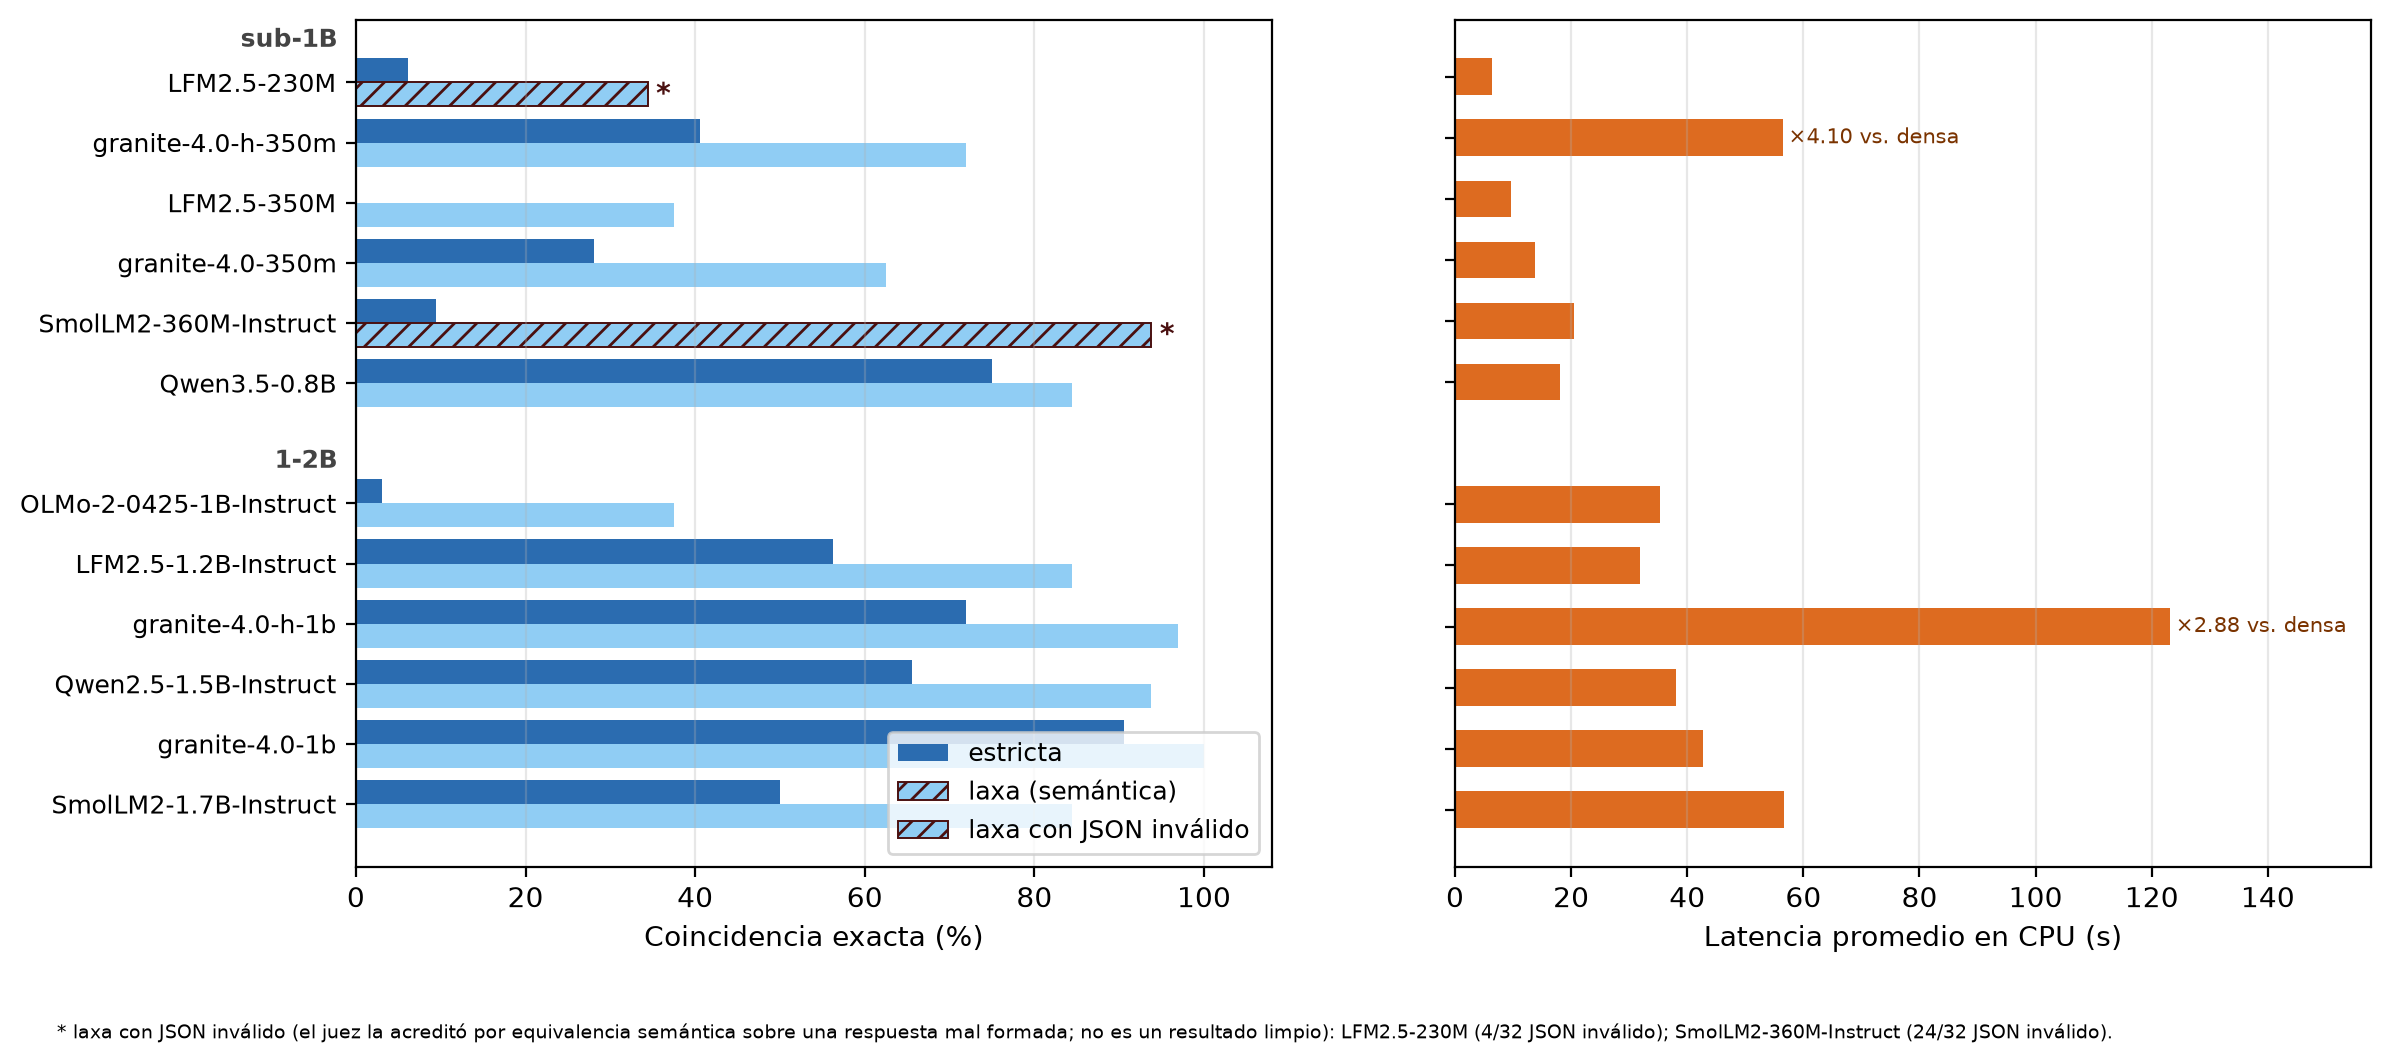
\includegraphics[width=\textwidth]{figuras/fig1_exactitud_latencia_2026.png}
\caption{Coincidencia exacta estricta y laxa (izquierda) y latencia promedio de
inferencia en CPU (derecha), por modelo, agrupados por tamaño.}
\label{fig:globales}
\end{figure}

El barrido principal se completó sobre los doce modelos del roster activo sin
ninguna falla irrecuperable: las 384 filas (12 modelos $\times$ 32 comandos) de
la Tabla \ref{tab:globales} están completas.

Bajo el prompt 2026 mantenido fijo a ambos lados de la comparación,
\texttt{granite-4.0-1b} alcanza \textbf{90,6\%} de exactitud estricta, la cifra
más alta de las doce evaluadas, frente al \textbf{65,6\%} de
\texttt{Qwen2.5-1.5B-Instruct}, el mejor modelo del brazo de generación
anterior medido idénticamente bajo ese mismo prompt: una diferencia de
\textbf{+25,0 puntos porcentuales}. En el otro extremo, \texttt{LFM2.5-350M}
no acierta ninguno de los 32 comandos bajo el protocolo estricto (0,0\%) pese a
emitir JSON válido en el 100\% de sus respuestas (Tabla \ref{tab:globales});
esa combinación se retoma en la Sección \ref{sec:analisis-errores} como fallo
semántico genuino, no como un artefacto de formato.

La ventaja del tier 1--2B sobre el tier sub-1B se sostiene en promedio, pero
no es universal: \texttt{Qwen3.5-0.8B}, el único modelo sub-1B con exactitud
estricta de tres dígitos de magnitud comparable a los mejores del tier
superior, supera en la Tabla \ref{tab:globales} a cuatro de los seis modelos
del tier 1--2B (\texttt{LFM2.5-1.2B-Instruct}, \texttt{OLMo-2-0425-1B-Instruct},
\texttt{SmolLM2-1.7B-Instruct} y \texttt{Qwen2.5-1.5B-Instruct}), y sólo queda
por debajo de las dos variantes de \texttt{granite-4.0} de mayor tamaño. Ese
desempeño, sin embargo, tiene un costo en latencia que no es uniforme dentro
del propio tier: la Sección \ref{sec:discusion-latencia-hibrida} discute en
detalle el caso de las variantes híbridas de \texttt{granite-4.0}, que
multiplican su latencia respecto de la variante densa del mismo tamaño sin
una ganancia de exactitud proporcional.

La Figura \ref{fig:globales} y la Tabla \ref{tab:globales} muestran además
que la brecha entre exactitud estricta y laxa es grande y desigual entre
modelos: en varios casos la exactitud laxa más que duplica a la estricta.
Esa brecha es, en sí misma, un resultado de este trabajo y no un simple
matiz — se retoma con el detalle por categoría de error en la Sección
\ref{sec:analisis-errores} y se discute en la Sección 5, porque parte de esa
brecha resulta poco confiable exactamente donde la validez de formato es
débil.

\textbf{Continuidad con la ronda inicial de este experimento.}
\label{sec:continuidad}
Tres de los doce modelos del roster activo —\texttt{SmolLM2-360M-Instruct},
\texttt{Qwen2.5-1.5B-Instruct} y \texttt{SmolLM2-1.7B-Instruct}— también
habían sido medidos en una ronda inicial de este mismo experimento (2025).
Para esos tres, y sólo para esos tres, la Tabla \ref{tab:globales} agrega
dos columnas de continuidad, ``Estricta 2025 (\%)'' y ``Latencia 2025 (s)'',
tomadas directamente de esa medición inicial; los otros nueve modelos
llevan un guion en esas dos columnas porque no tienen contraparte en esa
ronda. Comparando exclusivamente esas dos columnas contra las
correspondientes de este trabajo: la exactitud estricta de
\texttt{SmolLM2-360M-Instruct} desciende respecto de la medición inicial,
la de \texttt{Qwen2.5-1.5B-Instruct} sube, y la de \texttt{SmolLM2-1.7B-Instruct}
también desciende; en latencia, \texttt{SmolLM2-360M-Instruct} sube respecto
de la medición inicial mientras que \texttt{Qwen2.5-1.5B-Instruct} y
\texttt{SmolLM2-1.7B-Instruct} bajan. Ninguna de las tres cifras estrictas se
mueve en la misma dirección que las otras dos, lo que ya es un primer
indicio de que el modelo por sí solo no explica la diferencia; la
interpretación completa de este patrón, atribuido al protocolo y al arnés de
ejecución y no al modelo, se desarrolla en la Sección 5.

\subsection{Exactitud por campo del esquema}

\begin{figure}[htbp]
\centering
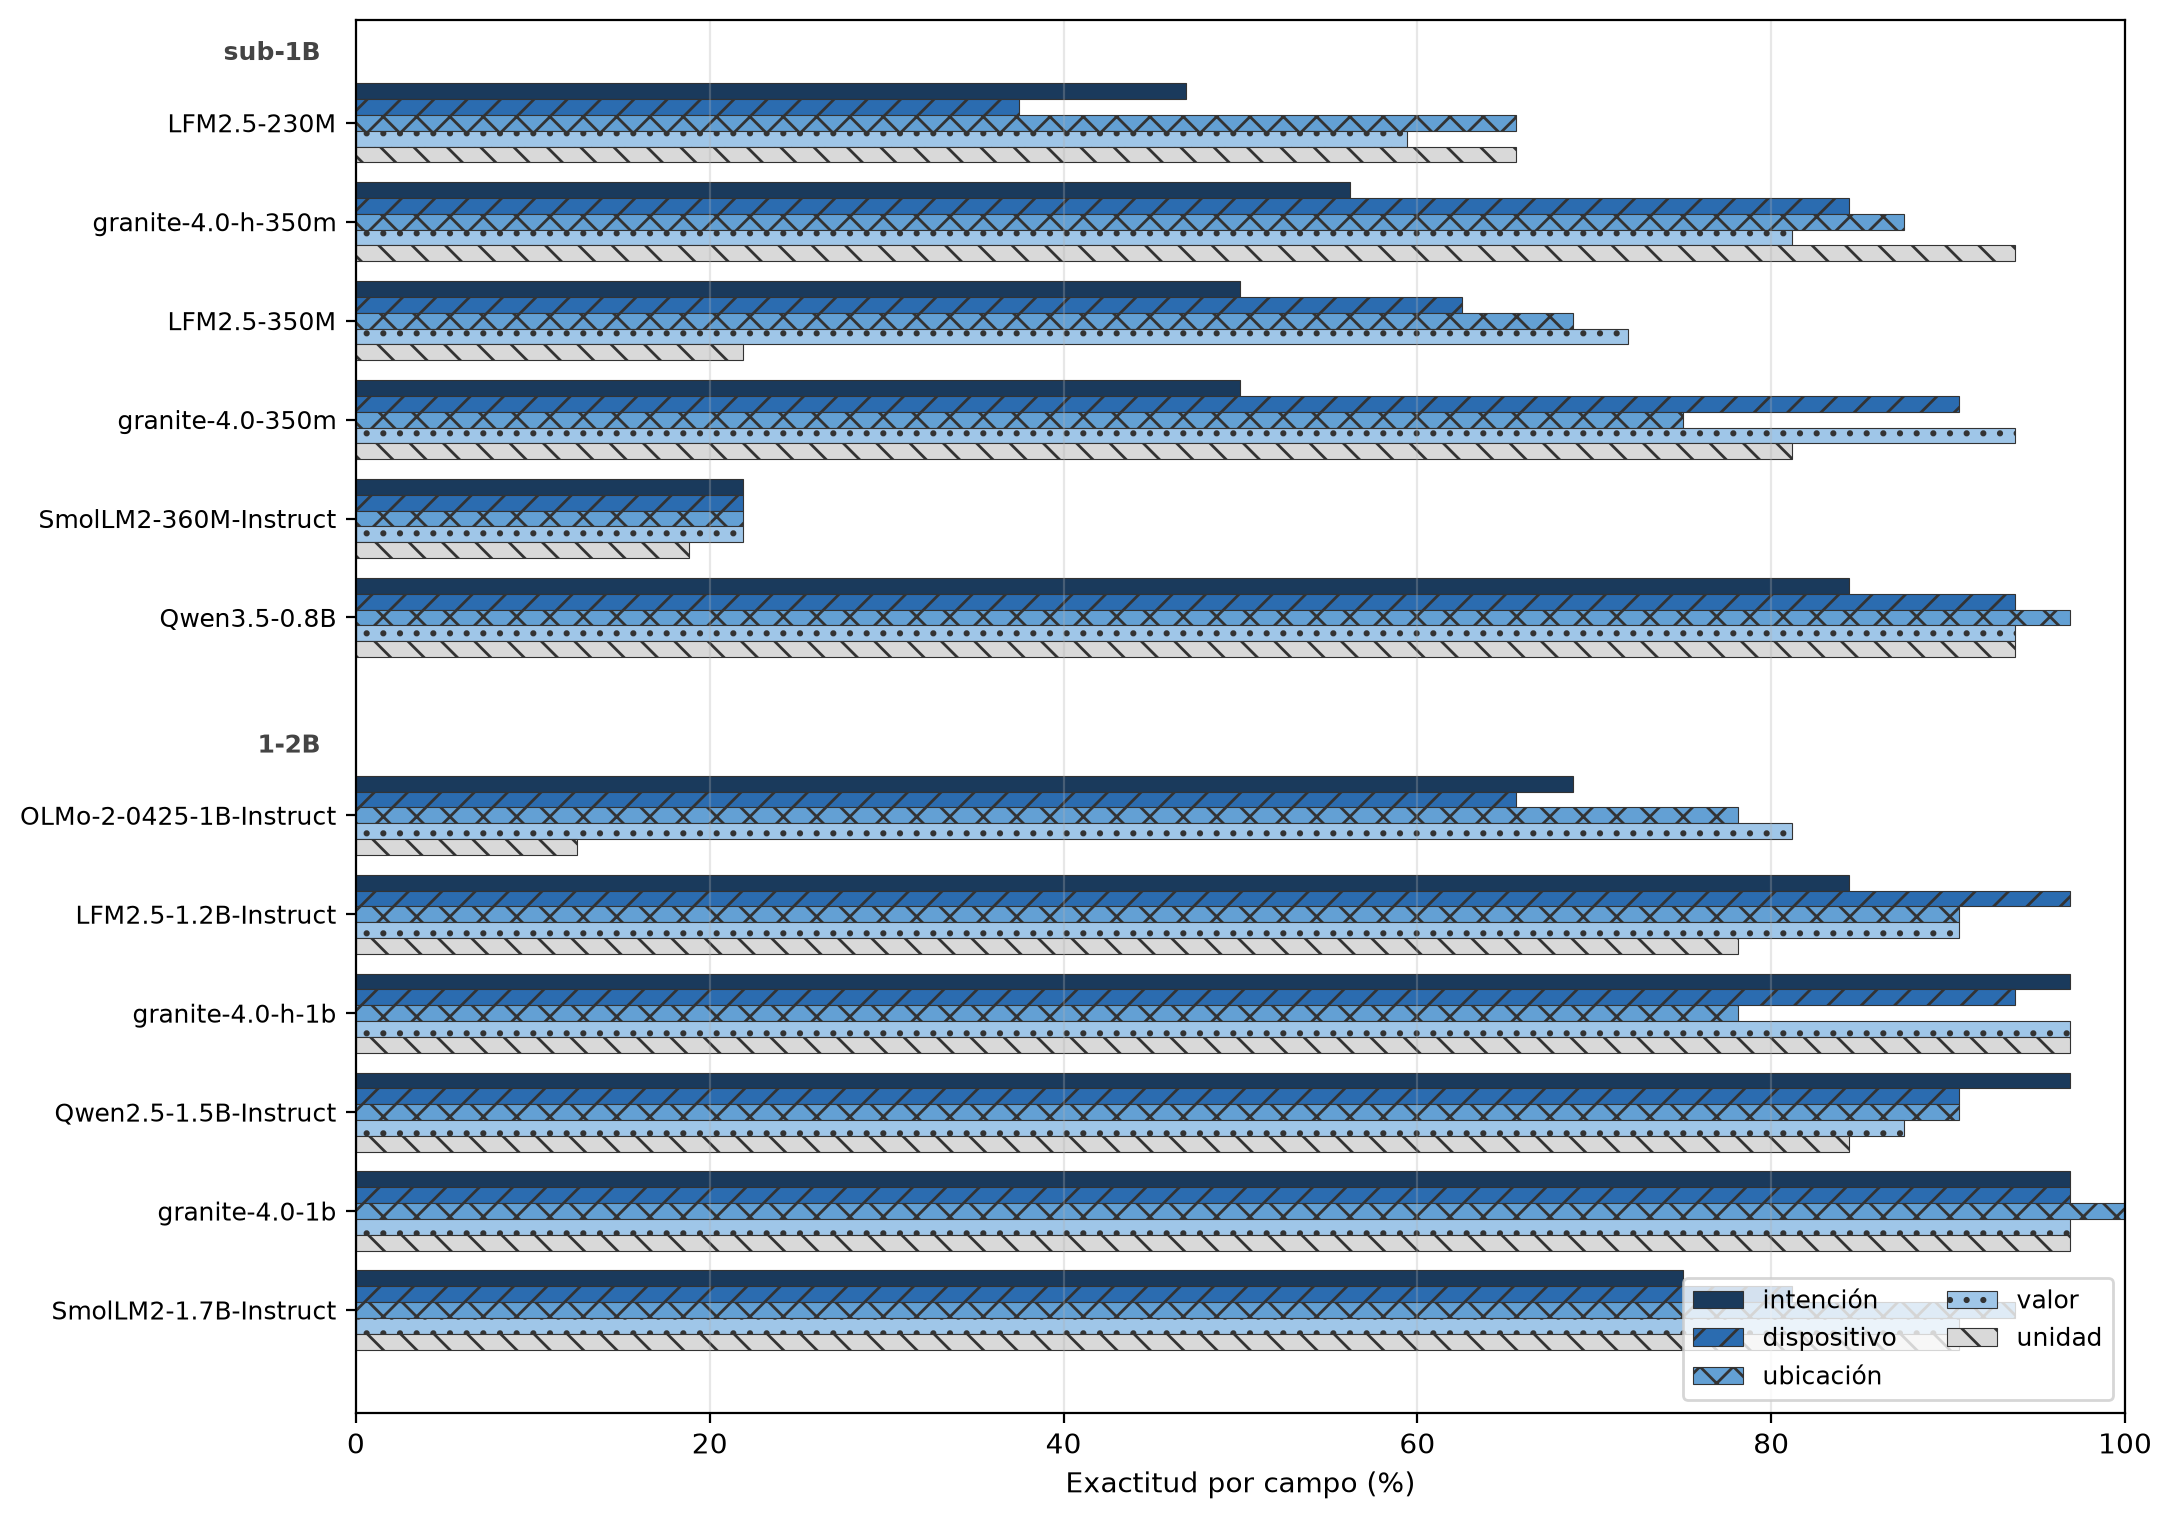
\includegraphics[width=\textwidth]{figuras/fig2_exactitud_por_campo_2026.png}
\caption{Exactitud por campo del esquema de salida (intent, dispositivo,
ubicación, valor, unidad), por modelo, agrupados por tamaño.}
\label{fig:campos}
\end{figure}

La Figura \ref{fig:campos} descompone la exactitud por cada uno de los cinco
campos del esquema de salida. Promediando sobre los doce modelos, el campo
\texttt{intent} y el campo \texttt{unidad} son los que concentran, en
promedio, la mayor tasa de error, mientras que \texttt{valor} y
\texttt{ubicacion} son los campos que los modelos resuelven de forma más
consistente. El campo \texttt{unidad} en particular muestra el rango más
amplio entre modelos: hay modelos que lo resuelven casi siempre y otros para
los que es, junto con \texttt{intent}, el campo menos confiable, lo que
sugiere que gran parte del error de exactitud estricta no proviene de una
confusión de intención grave sino de detalles de menor jerarquía semántica
del esquema (qué unidad o qué valor acompaña a un ajuste correctamente
identificado).

\subsection{Exactitud por categoría lingüística}

\begin{table}[htbp]
\centering
\caption{Exactitud estricta por categoría lingüística}
\label{tab:categorias}
\resizebox{\textwidth}{!}{%
\begin{tabular}{lrrrrrrrrrrrr}
\toprule
Categoría (n) & LFM2.5-230M & granite-4.0-h-350m & LFM2.5-350M & granite-4.0-350m & SmolLM2-360M-Instruct & Qwen3.5-0.8B & OLMo-2-0425-1B-Instruct & LFM2.5-1.2B-Instruct & granite-4.0-h-1b & Qwen2.5-1.5B-Instruct & granite-4.0-1b & SmolLM2-1.7B-Instruct \\
\midrule
Encendido / apagado simple (15) & 6.7 & 6.7 & 0.0 & 20.0 & 6.7 & 60.0 & 0.0 & 46.7 & 60.0 & 60.0 & 86.7 & 33.3 \\
Ajuste con valor numérico (14) & 7.1 & 78.6 & 0.0 & 35.7 & 7.1 & 92.9 & 7.1 & 71.4 & 92.9 & 78.6 & 100.0 & 71.4 \\
Ajuste relativo / cualitativo (3) & 0.0 & 33.3 & 0.0 & 33.3 & 33.3 & 66.7 & 0.0 & 33.3 & 33.3 & 33.3 & 66.7 & 33.3 \\
\bottomrule
\end{tabular}
}
\end{table}


Las categorías lingüísticas de la Tabla \ref{tab:categorias} no las asignó un
anotador humano, como en la ronda inicial de este experimento, sino el juez
automático descripto en la Sección \ref{sec:dos-etapas}, sobre el mismo
vocabulario cerrado de seis categorías del dataset original. La comparación
contra la distribución de esa ronda inicial (8/8/6/4/3/3 sobre las seis
categorías) revela una diferencia que no conviene ocultar: el juez automático, en esta corrida, sólo utilizó
tres de las seis categorías cerradas —\emph{encendido/apagado simple}
(15 comandos), \emph{ajuste con valor numérico} (14) y \emph{ajuste relativo o
cualitativo} (3)— y ninguno de los 32 comandos quedó clasificado en
\emph{múltiples dispositivos}, \emph{consulta de estado} ni \emph{negación o
contexto conversacional}. Una inspección de las asignaciones muestra el patrón
del colapso: comandos que preguntan por un estado (``¿Está prendida la luz del
living?''), que niegan una acción previa (``No dejes prendida la luz de la
cocina, apagala'') o que involucran varios dispositivos a la vez (``Apagá
todas las luces de la casa'') quedaron plegados dentro de
\emph{encendido/apagado simple} o de \emph{ajuste relativo o cualitativo} en
lugar de formar sus propias categorías. Esto no afecta la exactitud estricta
ni laxa, que se calculan por comando y no dependen de la categoría asignada,
pero sí limita el valor de la Tabla \ref{tab:categorias} como desagregación
lingüística fina en esta corrida, y se retoma como una limitación de la
asignación automática de categoría en la Sección 6.

\subsection{Análisis automático de errores}
\label{sec:analisis-errores}

\begin{table}[htbp]
\centering
\caption{Distribución de errores por categoría de la taxonomía}
\label{tab:taxonomia}
\resizebox{\textwidth}{!}{%
\begin{tabular}{lrrrrrrrrrrrr}
\toprule
Categoría de error & LFM2.5-230M & LFM2.5-350M & granite-4.0-350m & granite-4.0-h-350m & Qwen3.5-0.8B & SmolLM2-360M-Instruct & LFM2.5-1.2B-Instruct & granite-4.0-1b & granite-4.0-h-1b & OLMo-2-0425-1B-Instruct & SmolLM2-1.7B-Instruct & Qwen2.5-1.5B-Instruct \\
\midrule
Total de respuestas incorrectas & 30 & 32 & 23 & 19 & 8 & 29 & 14 & 3 & 9 & 31 & 16 & 11 \\
Confusión de intención & 0 & 0 & 3 & 0 & 1 & 0 & 2 & 0 & 0 & 0 & 0 & 0 \\
Confusión de dispositivo & 20 & 20 & 9 & 9 & 4 & 2 & 3 & 0 & 1 & 19 & 5 & 1 \\
Confusión de ubicación & 4 & 5 & 0 & 0 & 0 & 0 & 0 & 0 & 0 & 3 & 0 & 1 \\
Alucinación de valor/unidad & 0 & 0 & 0 & 0 & 0 & 0 & 0 & 0 & 0 & 0 & 0 & 0 \\
Valor numérico incorrecto & 0 & 0 & 0 & 0 & 0 & 0 & 0 & 0 & 0 & 1 & 0 & 0 \\
Sin error semántico & 1 & 1 & 5 & 3 & 0 & 1 & 2 & 1 & 7 & 2 & 5 & 2 \\
Uso de sinónimos & 8 & 11 & 6 & 7 & 3 & 26 & 7 & 2 & 1 & 9 & 6 & 7 \\
\bottomrule
\end{tabular}
}
\end{table}


Esta subsección reemplaza la revisión manual de respuestas incorrectas de la
ronda inicial de este experimento por una clasificación completamente
automática. El juez es el
modelo seleccionado por la regla congelada de la Sección \ref{sec:dos-etapas}
—mayor exactitud estricta de la etapa 1, empate hacia el modelo de mayor
tamaño—, que en este barrido es \texttt{granite-4.0-1b}, con \textbf{90,6\%}
de exactitud estricta en la etapa 1 (el mismo valor que su exactitud estricta
final, porque no cambia entre etapas). Cada una de las 225 respuestas con
\texttt{match\_exact = False} se clasificó en un subconjunto no vacío de las
\textbf{siete} etiquetas de la Tabla \ref{tab:taxonomia} —las cinco heredadas
de la ronda inicial de este experimento, con \emph{alucinación de valor/unidad} y \emph{valor
numérico incorrecto} ya separadas en dos etiquetas distintas en vez de
fusionadas en una, más \emph{sin error semántico} y \emph{uso de sinónimos},
que son precisamente las que definen la exactitud laxa—. Ninguna de las 225
respuestas clasificadas, ni ninguna de las 32 asignaciones de categoría
lingüística de la Sección 4.3, quedó con \texttt{juez\_parse\_ok = False}: el
juez no necesitó ningún reintento ni ninguna etiqueta de respaldo en esta
corrida.

La métrica laxa rescató, en conjunto, \textbf{123} de las 225 respuestas
incorrectas bajo el protocolo estricto (etiquetadas \texttt{sin\_error\_semantico}
o \texttt{uso\_de\_sinonimos}), es decir algo menos de un tercio de las 384
respuestas totales del barrido. Un ejemplo puntual, relevante para la Sección
5: de las 30 respuestas incorrectas de \texttt{LFM2.5-230M}, \textbf{9} son
\texttt{uso\_de\_sinonimos} o \texttt{sin\_error\_semantico} — casi un tercio
de sus errores estrictos no son errores de contenido sino de vocabulario.

La Tabla \ref{tab:taxonomia} por sí sola no distingue, sin embargo, entre dos
formas muy distintas de tener exactitud estricta cercana a cero, y esa
distinción es un requisito de este trabajo: un \texttt{json\_valido} alto
junto a una exactitud casi nula indica que el modelo emite el formato
correctamente y se equivoca en el contenido —un fallo semántico genuino, y un
resultado en sí mismo—, mientras que un \texttt{json\_valido} bajo junto a una
exactitud casi nula indica que el modelo ni siquiera logra emitir el formato
—un artefacto de parseo, no una incapacidad semántica—. Sobre la Tabla
\ref{tab:globales}: \texttt{LFM2.5-350M} tiene 0,0\% de exactitud estricta con
\textbf{100\%} de JSON válido, y \texttt{OLMo-2-0425-1B-Instruct} tiene 3,1\%
de exactitud estricta con también \textbf{100\%} de JSON válido — ambos son,
por lo tanto, fallos semánticos genuinos. \texttt{SmolLM2-360M-Instruct}, en
cambio, tiene 9,4\% de exactitud estricta pero sólo \textbf{25\%} de JSON
válido: su exactitud casi nula es, en buena medida, un artefacto de formato, y
tratarla como incapacidad semántica contaminaría la conclusión. Por esta razón
la afirmación de ``100\% de JSON válido'' de la ronda inicial de este
experimento no puede repetirse sin matices en este trabajo: con el roster
de doce modelos la validez de formato
no es universal (25\% en \texttt{SmolLM2-360M-Instruct}, 87,5\% en
\texttt{LFM2.5-230M}, y 100\% en los nueve modelos restantes).

Esta distinción tiene además una consecuencia directa sobre la confiabilidad
de la propia métrica laxa, que conviene declarar aquí explícitamente en vez de
como una nota al pie: la métrica laxa es poco confiable exactamente donde la
validez de formato es débil. El campo \texttt{laxo\_json\_invalido\_n} —el
número de respuestas que el juez etiquetó \texttt{sin\_error\_semantico} o
\texttt{uso\_de\_sinonimos} (y que por lo tanto cuentan para la exactitud laxa)
pese a que su JSON no era válido— es \textbf{24} para
\texttt{SmolLM2-360M-Instruct}, sobre apenas \textbf{27} respuestas rescatadas
en total por la métrica laxa para ese modelo: es decir que 24 de esas 27
respuestas ``semánticamente equivalentes'' tenían JSON inválido, y el juez las
acreditó de todos modos. Su exactitud laxa de 93,8\% es, en consecuencia, un
artefacto de la fragilidad de formato de este modelo, no evidencia de
competencia semántica. El mismo campo vale \textbf{4} para
\texttt{LFM2.5-230M} (sobre 9 respuestas rescatadas) y \textbf{0} para los diez
modelos restantes. Esta amenaza a la confiabilidad de la métrica laxa se
retoma en la Sección 6.
